\chapter[Cognitive Radio]{Cognitive Radio}
%\addcontentsline{toc}{chapter}{Chapter 1\\Introduction}
\label{chapter:CR}
In Chapter \ref{chapter:CR}, cognitive radio technology for spectrum sharing is described in detail. Also, as one of the applied technology, spectrum sharing with spectrum database is discussed.

\section{Overview of Cognitive Radio}
Cognitive Radio(CR) is defined as the technology that wireless communication devices are able to be aware of the surrounding environment and configure communication parameters autonomously. Frequency in use, Modulation method, Transmission power all can be treated as communication paramters. Because the adaptive parameter configuration can make an effective usage on White Space possible, it is expected as a solution to the shortage of the spectrum resources.

As a process for Secondary User communication, a series of algorithm named as Cognitive Cycle\cite{ref:mitola} is proposed by J.Mitola I\hspace{-.1em}I\hspace{-.1em}I in 1999. With observing Outside World, Secondary User can obtain various informaiton. Next, after analysis is executed based on information from observation, results are oriented by priority and process is carried out depending on the determined oriented result. If the status has to be responded instantaneously, the appropriate Act needs to be reacted immediately with using the information obtained. For example, when the status of Primary User changes to ON, Secondary User has to stop transmission immediately. Otherwise, in the case that an urgent status exists, an act needs to be determined based on the information. As an example, when Secondary User has an effect on primary signal with huge interfernce power, it is necessary to move to the phase which is stopping transmission or lower the interferece power. If the priority is Normal, an optimised Plan is determined with a long-term observation. While the radio environment changes, the obversation will be observered again. At the end, the Cognitive Cycle is possible based on the process below.
\begin{figure}[!htp]
\begin{center}
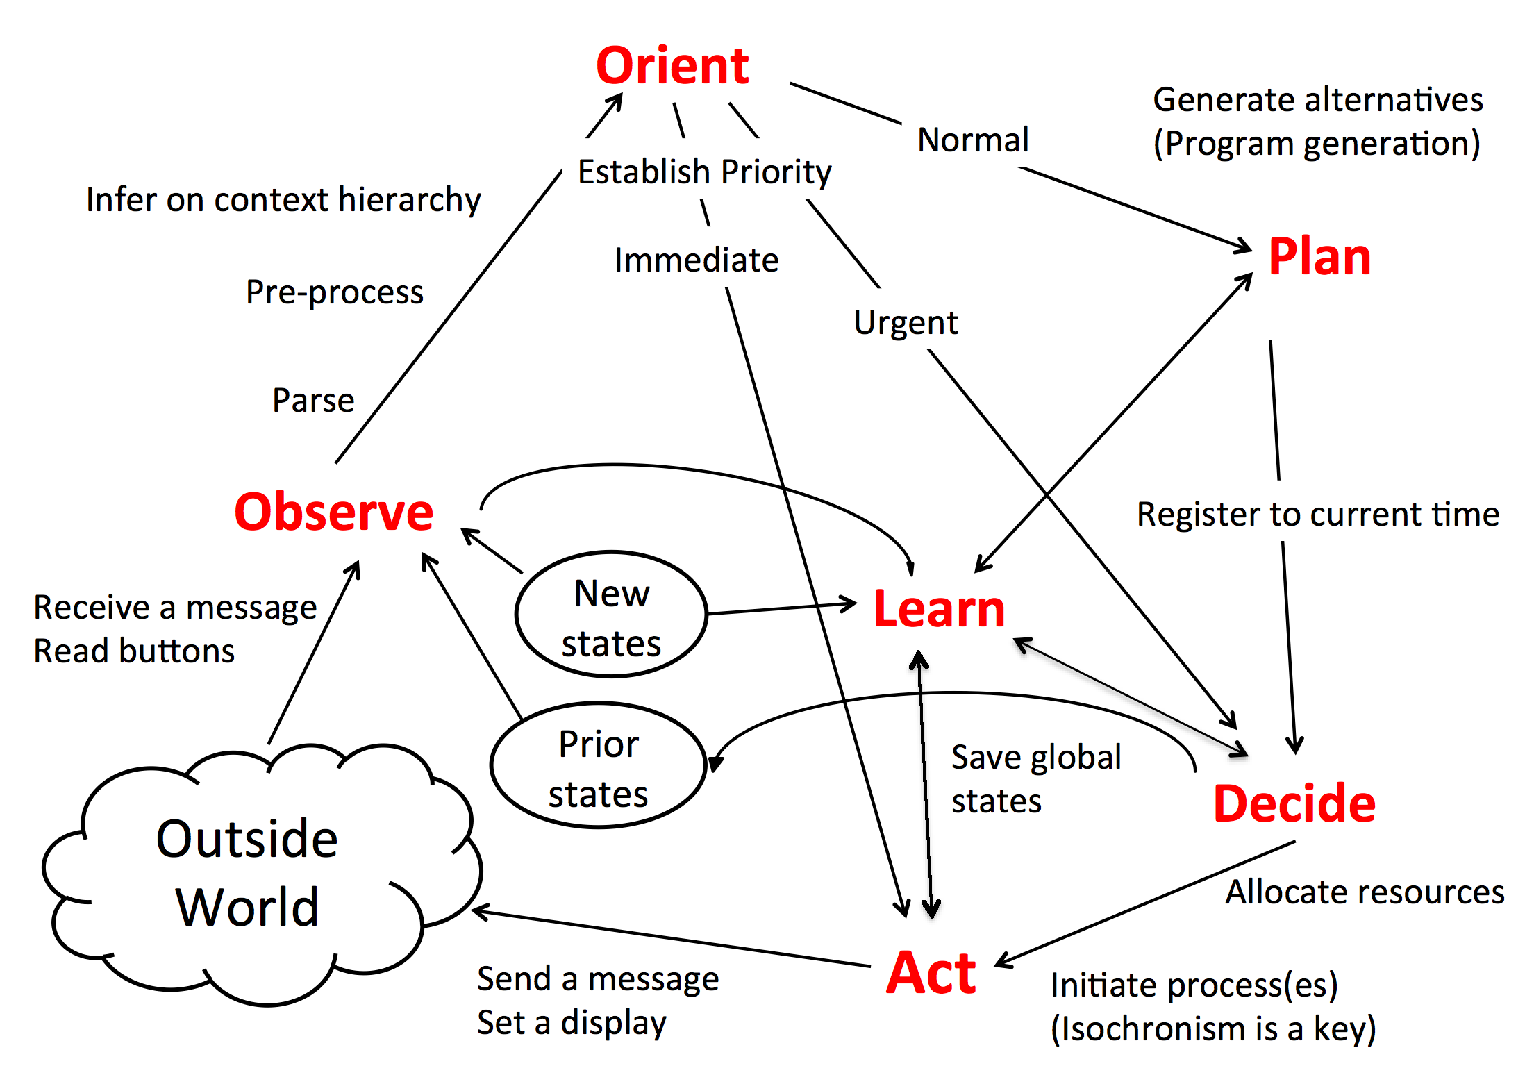
\includegraphics[width=100mm,clip]{cognitive_cycle.eps}
\caption{Cognitive Cycle.}
\label{fig:cognitive cycle}
\end{center}
\end{figure}

The protection of Primary transmission is related to the observation and determination. The signal from Primary User, the own location information from Global Position System(GPS), and the sensing infromation from other nodes can be treated as the observation data. Next, the determination process is optimally executed according to the observation data. Whether the Primary User existence can be determined accurately plays an key role to the cognitive radio sysytems.

In this thesis, we focus on the observe and Orient process in the cognitive cycle for our proposed method.

\section{Multi-mode System}
Cognitive Radio technology which is researched actively is roughly divided into two tpyes: Multi-mode System and Dynamic Spectrum Access. In Multi-mode System as illustrated in Fig. \ref{fig:hetero}, Secondary User is allowed to detect the temporally and spatially unused licensed band and utilize the spectrum with same behavior as Primary User. If the Quality of Service(QoS) is not able to be achieved from the certain spectrum band, Secondary User switches to another spectrum. While Multimode system is realized as a easier method than Dynamic Spectrum Access with the reason that the communication method has already been established, the spectrum usage efficiency is not remarkable due to the upper limitation on the communication scheme of Primary User.

\begin{figure}[!htp]
\begin{center}
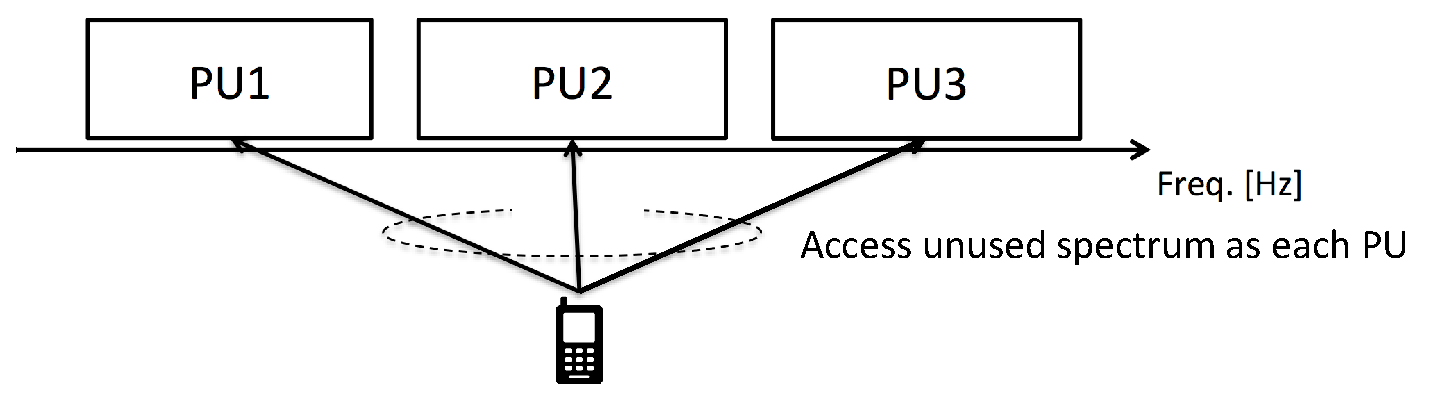
\includegraphics[width=100mm,clip]{multimode.eps}
\caption{Multi-mode System.}
\label{fig:hetero}
\end{center}
\end{figure}

\section{Dynamic Spectrum Access for Spectrum Sharing}
As Dynamic Spectrum Access is possible for more flexible spectrum utilization, huge spectrum usage efficency improvement In the Dynamic Spectrum Access, Secondary Users are able to detect the spectrum and access to it with lower priority than Primary User of that spectrum. As a constraint, harmful interference toward Primary User is not allowed. The method about how to access to the spectrum is composed of two types, which is defined as Overlay Spectrum Sharing\cite{ref:overlay} and Underlay Spectrum Sharing\cite{ref:underlay}.

\subsection{Overlay Spectrum Sharing}
As illustrated in Fig.\ref{fig:overlay}, Unused White Space is utilized for communication in Overlay Spectrum Sharing. If the existence of Primary User in this spectrum is accurately detected by Secondary User, the protection of Primary User will be possible and the opportunity for Secondary User can be gained. In other words, the detection method on Primary User is  the way to achieve Overlay Spectrum Sharing.
    
\begin{figure}[!htp]
\begin{center}
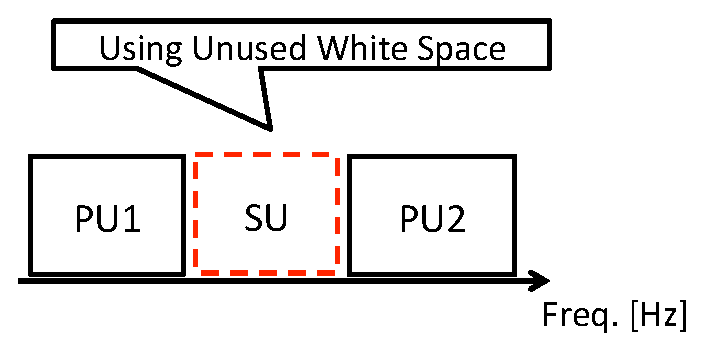
\includegraphics[width=100mm,clip]{overlay.eps}
\caption{Overlay Spectrum Sharing.}
\label{fig:overlay}
\end{center}
\end{figure}

\subsection{Underlay Spectrum Sharing}
 Difference with Overlay Spectrum Sharing, licenced band for Primary User is considered as In other words, Both Primary User protection and own performance with using appropriate communication method should be ensured.
\begin{figure}[!htp]
\begin{center}
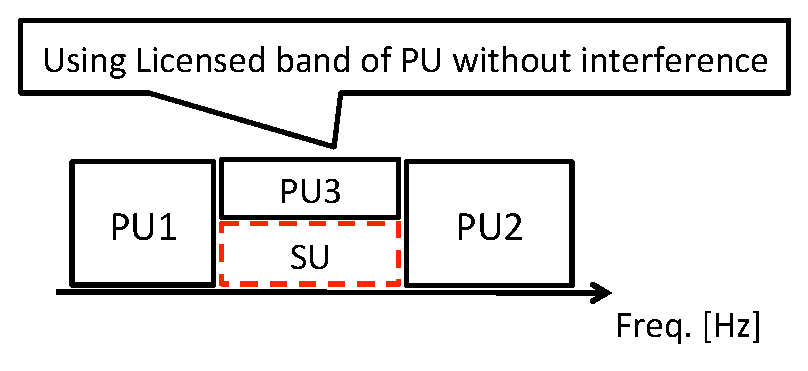
\includegraphics[width=100mm,clip]{underlay.eps}
\caption{Underlay Spectrum Sharing.}
\label{fig:underlay}
\end{center}
\end{figure}

\section{Overview of Spectrum Sharing with Spectrum Database}
